\section{Number of fields per cell: distribution fits}
\label{sec:field_count}
\noindent\textit{Analysis \texttt{field\_count}, 38 sessions, fingerprint \texttt{c0c66d121108}.}

1{,}881 of 2{,}515 good pyramidal units were place cells (37 sessions, 2 rats); they had 12.79 fields on average (median 9, range 1--72; Table~\ref{tab:field_count:summary}). \textbf{Detector noise floor:} spike-shift surrogates of the same cells (spatial tuning destroyed, rate and sampling preserved) yield 14.54 fields per cell, against 12.79 observed; 34\% of cells have more fields than their own surrogates. Under the present detection criteria the field count is therefore dominated by firing rate and sampling noise rather than by the number of genuine place fields, and the shape of the distribution below should be read with that in mind.

\begin{itemize}
\item \textbf{pooled}: best model by AIC is the log-normal (discretised) (Akaike weight 1.00); Gaussian (discretised) $\Delta$AIC $= 107.0$, negative binomial (ZT) $\Delta$AIC $= 86.9$, Poisson (ZT) $\Delta$AIC $= 12319.2$.
\item \textbf{Rat5}: best model by AIC is the log-normal (discretised) (Akaike weight 1.00); Gaussian (discretised) $\Delta$AIC $= 72.6$, negative binomial (ZT) $\Delta$AIC $= 67.2$, Poisson (ZT) $\Delta$AIC $= 5179.4$.
\item \textbf{Rat6}: best model by AIC is the log-normal (discretised) (Akaike weight 1.00); Gaussian (discretised) $\Delta$AIC $= 48.0$, negative binomial (ZT) $\Delta$AIC $= 24.2$, Poisson (ZT) $\Delta$AIC $= 6734.1$.
\item Note on the Gaussian: its maximum-likelihood mean lies below the support ($\mu = -587$ fields), so only the upper tail of the bell is used and the fit is close to a geometric decay rather than a symmetric distribution around a typical count.
\item Goodness of fit: the best pooled model (log-normal (discretised)) is itself rejected, so it is the best of the candidates rather than a complete description (Pearson $\chi^2_{50} = 93.2$, $p = 2.04\times10^{-4}$; Table~\ref{tab:field_count:fits}).
\end{itemize}

\begin{table}[htbp]
\centering
\footnotesize
\caption{Fields per place cell, by rat. Fano = variance/mean ($>1$: over-dispersed relative to Poisson). Surrogate = same cells with circularly shifted spikes.}
\label{tab:field_count:summary}
\begin{tabular}{lrrrrrrrrr}
\toprule
rat & place cells & sessions & mean & median & variance & surrogate mean & surrogate median & Fano & frac.\ $>$ surrogate \\
\midrule
Rat5 & 880 & 18 & 10.9 & 7 & 128 & 12.9 & 9 & 11.7 & 0.302 \\
Rat6 & 1{,}001 & 19 & 14.4 & 10 & 170 & 15.9 & 11 & 11.8 & 0.369 \\
\bottomrule
\end{tabular}
\end{table}
\begin{table}[htbp]
\centering
\footnotesize
\caption{Maximum-likelihood fits to the number of fields per place cell ($k\geq1$). Models are sorted by AIC within each group. $\chi^2$: Pearson goodness of fit with counts pooled to an expected frequency $\geq5$.}
\label{tab:field_count:fits}
\begin{tabular}{llrrrrrrrrr}
\toprule
group & model & $n$ & params & $\ln L$ & $\Delta$AIC & $\Delta$BIC & weight & $\chi^2$ & dof & $p_{\mathrm{GOF}}$ \\
\midrule
pooled & log-normal (discretised) & 1{,}881 & 2 & -6546 & 0 & 0 & 1 & 93.17 & 50 & $2.04\times10^{-4}$ \\
pooled & negative binomial (ZT) & 1{,}881 & 2 & -6589 & 86.88 & 86.88 & $1.37\times10^{-19}$ & 188 & 46 & $4.53\times10^{-19}$ \\
pooled & geometric & 1{,}881 & 1 & -6599 & 104.2 & 98.61 & $2.42\times10^{-23}$ & 197.4 & 49 & $1.04\times10^{-19}$ \\
pooled & Gaussian (discretised) & 1{,}881 & 2 & -6599 & 107 & 107 & $5.78\times10^{-24}$ & 200.7 & 48 & $1.43\times10^{-20}$ \\
pooled & Poisson (ZT) & 1{,}881 & 1 & -12706 & 12319 & 12314 & 0 & 35480 & 19 & 0 \\
Rat5 & log-normal (discretised) & 880 & 2 & -2906 & 0 & 0 & 1 & 43.18 & 34 & 0.1345 \\
Rat5 & negative binomial (ZT) & 880 & 2 & -2940 & 67.22 & 67.22 & $2.53\times10^{-15}$ & 118 & 34 & $3.34\times10^{-11}$ \\
Rat5 & geometric & 880 & 1 & -2941 & 68.2 & 63.42 & $1.55\times10^{-15}$ & 112.3 & 35 & $4.89\times10^{-10}$ \\
Rat5 & Gaussian (discretised) & 880 & 2 & -2942 & 72.61 & 72.61 & $1.71\times10^{-16}$ & 117.2 & 34 & $4.56\times10^{-11}$ \\
Rat5 & Poisson (ZT) & 880 & 1 & -5497 & 5179 & 5175 & 0 & 6520 & 15 & 0 \\
Rat6 & log-normal (discretised) & 1{,}001 & 2 & -3612 & 0 & 0 & 1 & 85.08 & 44 & $2.00\times10^{-4}$ \\
Rat6 & negative binomial (ZT) & 1{,}001 & 2 & -3624 & 24.24 & 24.24 & $5.46\times10^{-6}$ & 113.5 & 42 & $1.71\times10^{-8}$ \\
Rat6 & Gaussian (discretised) & 1{,}001 & 2 & -3635 & 47.99 & 47.99 & $3.79\times10^{-11}$ & 135.3 & 44 & $3.19\times10^{-11}$ \\
Rat6 & geometric & 1{,}001 & 1 & -3638 & 50.72 & 45.81 & $9.69\times10^{-12}$ & 139.9 & 46 & $2.04\times10^{-11}$ \\
Rat6 & Poisson (ZT) & 1{,}001 & 1 & -6980 & 6734 & 6729 & 0 & 12479 & 18 & 0 \\
\bottomrule
\end{tabular}
\end{table}
\begin{table}[htbp]
\centering
\small
\caption{Dependence of field count on firing rate and training day (Spearman, place cells).}
\label{tab:field_count:confounds}
\begin{tabular}{lrrr}
\toprule
test & rho & p & n \\
\midrule
n\_fields \textasciitilde{} mean\_hz (Spearman) & 0.745 & 0 & 1{,}881 \\
n\_fields \textasciitilde{} day (Spearman) & -0.0886 & $1.19\times10^{-4}$ & 1{,}881 \\
n\_fields \textasciitilde{} surrogate n\_fields (Spearman) & 0.796 & 0 & 1{,}881 \\
surrogate n\_fields \textasciitilde{} mean\_hz (Spearman) & 0.828 & 0 & 1{,}881 \\
\bottomrule
\end{tabular}
\end{table}

\begin{figure}[htbp]
\centering
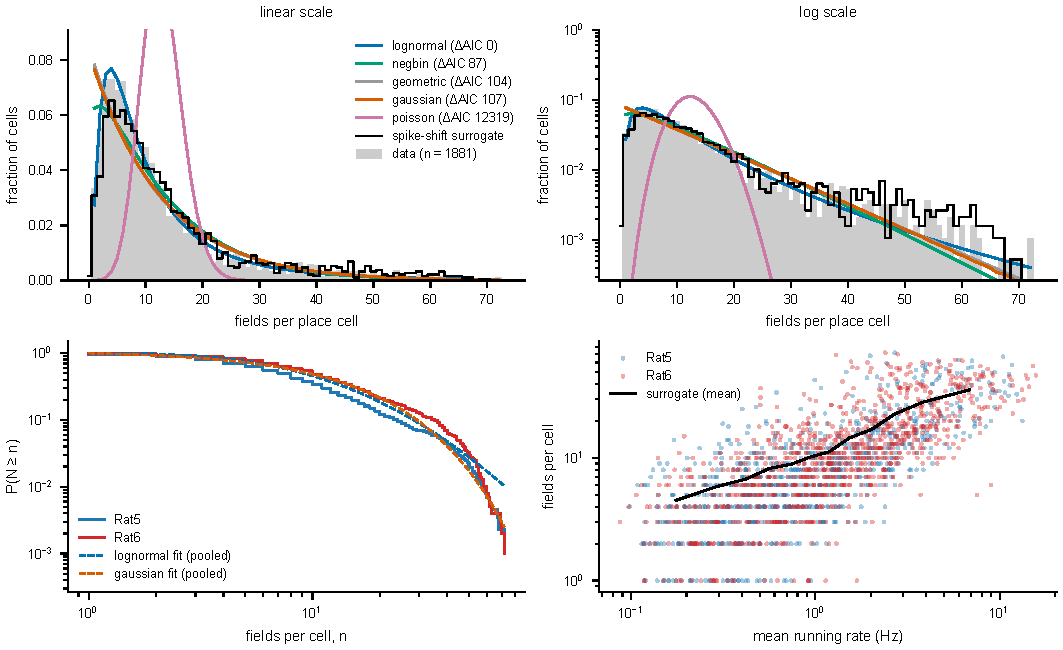
\includegraphics[width=\textwidth]{field_count__field_count.pdf}
\caption{\textbf{Fields per place cell.} Top: distribution over all place cells (bars) with the maximum-likelihood fit of each candidate model, on a linear (left) and logarithmic (right) $y$-axis; $\Delta$AIC relative to the best model in the legend. Bottom left: survival function $P(N\geq n)$ per rat on log--log axes with the pooled log-normal and Gaussian fits (dashed). Bottom right: field count against mean running rate, one dot per place cell. Black: the same cells after circularly shifting their spikes in time (spatial tuning destroyed, rate and maze sampling preserved), i.e.\ the noise floor of the field detector.}
\label{fig:field_count}
\end{figure}

\clearpage